
\documentclass{article}
\usepackage{ucs}
\usepackage[utf8x]{inputenc}
\usepackage[T1]{fontenc}

\usepackage{graphicx}
\usepackage{tipa}

\begin{document}
\title{Mo oažžut dihtora hálddašit lunddolaš giela válljenvejolašvuođaid giellaoahppanproseassas? \\ Gielalaš ja pedagogalaš čuolmmat.}   
\author{Lene Antonsen, Biret Ánne Bals Baal, \\ Saara Huhmarniemi, Trond Trosterud \\ \begin{figure}  \scalebox{0.10}[0.10]{
\includegraphics{img/LogoSamisk}} \end{figure}} 
\date{} 


\frame{\titlepage} 

%\frame{\frametitle{Table of contents}\tableofcontents} 

\section{Álggahus}
\subsection{VISL-prográmmat
\subsection{OAHPA-prográmmat}
- eará sámegiel. progr?

\section{Giellateknologiija}
- vejolaččat - Let´s Chat - multiple choice
- string match
- mo CG doaibmá
- min systema

Morfa?

\section{Vasta}
\subsection{Mo doaibmá}
- task genereren
- ekskl.pronomen

\section{Sahka}
\subsection{Mo doaibmá}
- inklus.pronomen
- čállojuvvon jearaldagat
- no random
- logihkka vástadusa ektui


\section{Cuolmmat   }
- lunddolaš vai ped?

feedbacka grammatihka vuođul:
- finihtta vearbbat
- nom vs akk

čállinmeattáhusaid bagadeapmi
-----------------------------
- dovdameahttun sátni -
	1. "tastefeil" 
	2. sojahanfeaila
	- álki addit čállinfeailafeedback
	- váttis bagadit geavaheaddji 
		1. gehčosa bokte livččii vejolaš kommenteret
		2. iskat lonuhit a/á 
		3. ped.divvun livččii vejolaš
- áiggukeahtes sátni -
	- váttis addit čállinfeailafeedback
	- vejolaš bagadit
	lok
	ill (báddii)
	biehttalanhápmi
	ordnetlohku vs. Nom.Pl. (viđát vs. viđat)


\section{vejolašvuođat ja konklušuvdna}
- semantalaš rollat?
boahtteáiggis: diehtovuorká ?
Oahpa-divvun-systema ?


%\section{Section no.1} 

\frame{\frametitle{ }
\begin{block}{ }
\textit{http://giellatekno.uit.no/oahpa/}\\
\end{block}{ }
Sámediggi ja Romssa Universitehta leat ruhtadan barggu
}

\frame{\frametitle{VISL-prográmmat}
\begin{block}{ }
\textbf{Oahppat grámmatihka:}\\
\end{block}{ }
Sátneluohkáid, syntávssa.
}

\frame{\frametitle{OAHPA-prográmmat}
\begin{block}{ }
\textbf{Oahppat sámegiela:}\\
\end{block}{}
\begin{itemize}
\item \textbf{Leksa}: Sátnequiz - sámi/dáru ja dáru/sámi
\item  \textbf{Numra}: Hárjehallat loguid
\item  \textbf{Morfa}: Hárjehallat sojahit sániid, maid konteavsttas
\item  \textbf{Vasta}: Hárjehallat vástidit jearaldagaide
\item  \textbf{Sahka}: Hárjehallat ságastallat dihto fáttás
\end{itemize}
}

\frame{\frametitle{Pedagogalaš prográmmat}
Pedagogalaš prográmmain ii leat dábálaččat giellateknologiija, muhto
\begin{itemize}
\item multiple choice 
\item stringmatch, omd \textit{viesus} = 6 mearkka: v i e s u s
\end{itemize} \pause
\begin{block}{ }
Giellateknologiija:
\begin{itemize}
\item analysa, omd \textit{viesus} = \textit{viessu} N Sg Loc
\end{itemize}
\end{block}{ }
}


\frame{\frametitle{Min áigumuš} 
Prográmma galgá bagadit geavaheaddji seammá ládje go oahpaheaddji dahká.
}

\frame{\frametitle{Vasta -- hárjehallat vástidit jearaldagaide} 
\scalebox{0.90}[0.90]{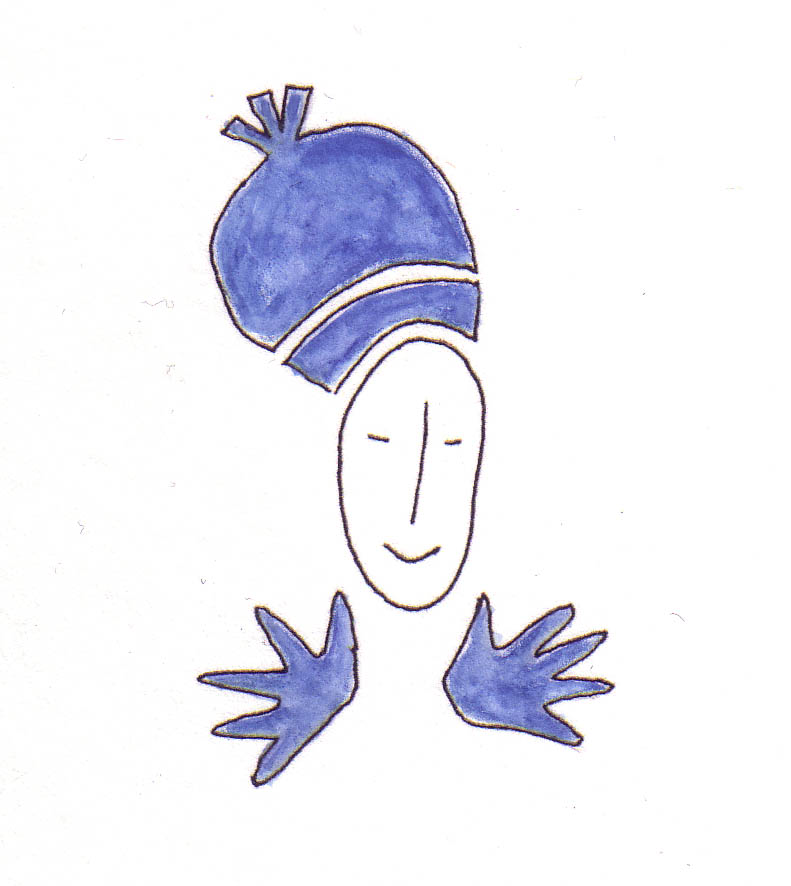
\includegraphics{img/vasta.png}} \\
}

\frame{\frametitle{Vasta} 
\scalebox{0.35}[0.35]{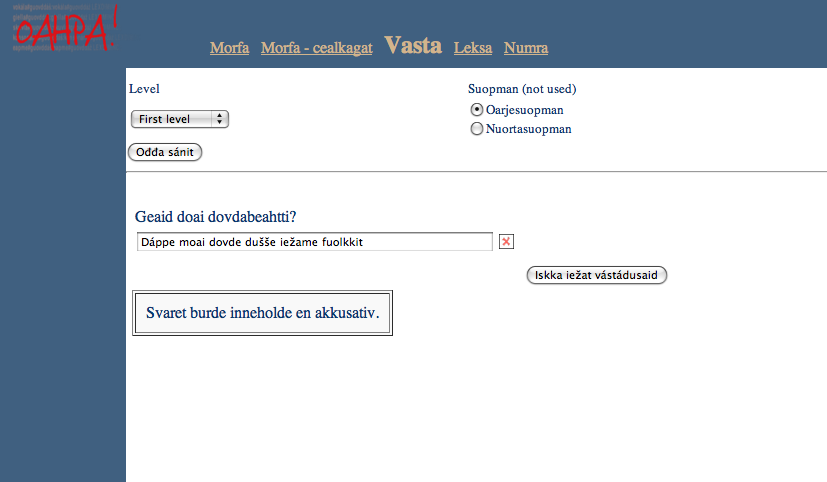
\includegraphics{img/vasta_jear.png}}
}


\frame{\frametitle{Maid don lohket ikte?} 

Dohkálaš vástádusat:
\begin{itemize}
\item Mun han lohken ollu áviissaid. 
\item Ikte mun gal lohken buori girjji. 
\item In lohkan maidege. 
\item Ikte in lohkan.
\end{itemize}
}

\frame{\frametitle{Maid don lohket ikte?} 

Vasta-prográmma bagada go vástádus ii leat dohkálaš:
\begin{itemize}
\item Mun lohket ollu áviissaid. \\ $\rightarrow$ Husk kongruens mellom subjekt og verbal.  
\item Mun lohken ollu áviissat. \\ $\rightarrow$ Objektet skal være i akkusativ. 
\item Don lohket ollu áviissaid. \\ $\rightarrow$ Er du sikker på at du svarer i riktig person?  
\end{itemize}
}

\frame{\frametitle{Min vuogádat} 
\scalebox{0.65}[0.65]{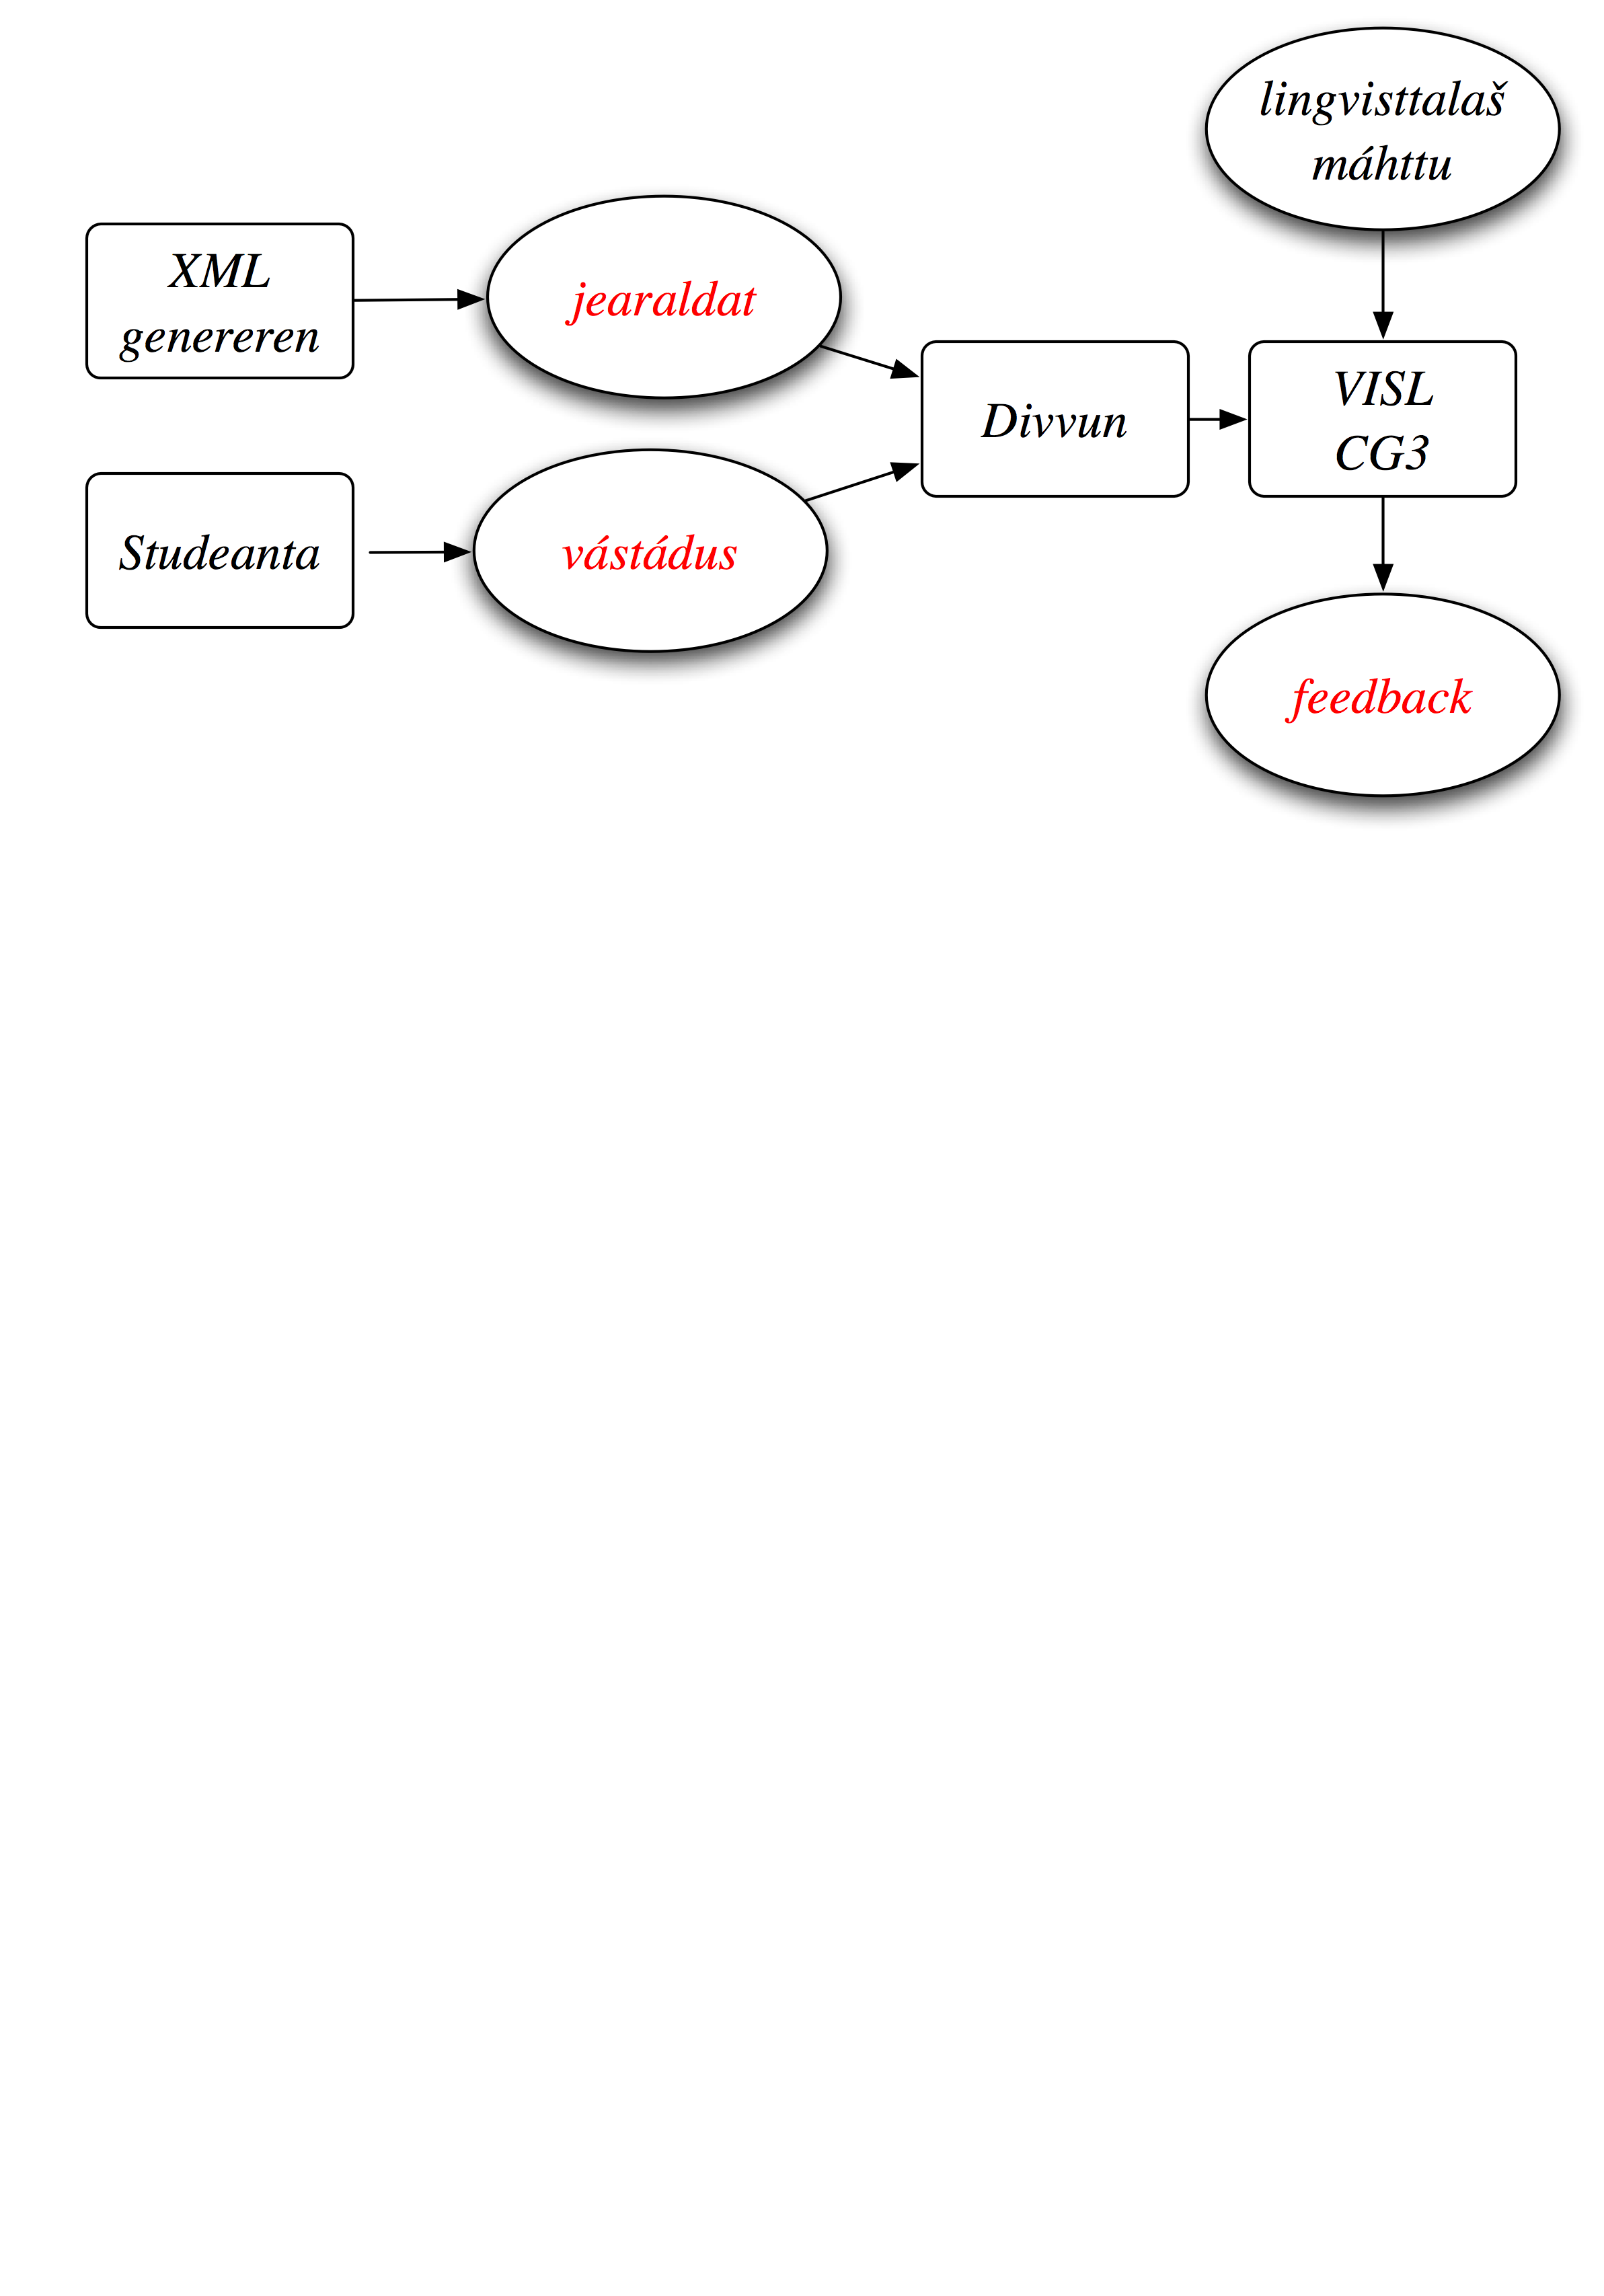
\includegraphics{img/skovi.png}} 
} 


\frame{\frametitle{Jearaldagaid genereren} 
      <text>Maid SUBJ MAINV ikte</text>
}

\frame{\frametitle{Lingvisttalaš máhttu} 
Mii geavahit min máhtu:
\begin{itemize}
\item sámegiela syntávssa birra		
\item ohppiid gaskagiela birra
\end{itemize}
}

\frame{\frametitle{Sámegiela syntáksa} 
omd. maid NP sáhttá sisttisdoallat:
\begin{itemize}
\item \small{NP $\rightarrow$ Pron A N Num Adv A CC Adv A N}  \\ 	
\textit{mu boares áhku guokte hui stuora ja hirbmat váralaš beatnaga}	
\item makkár kongruensa NP siskkobealde
\end{itemize}
}


\frame{\frametitle{Lunddolaš ságastallan}

\begin{description}
\item [ ] D: Siđat go gáfe?   G: In dieđe vuos. \pause 
\item [ ] $\rightarrow$ Det er for enkelt å svare vet-ikke. Prøv igjen. \pause 
\item [ ] D: Maid háliidat borrat?   G: Láibbi. \pause 
\item [ ] $\rightarrow$ Svaret ditt må alltid inneholde et finitt verb. \pause 
\item [ ] D: Áiggut go vázzit bargui odne?   G: Ale jeara nu olu. \pause 
\item [ ] $\rightarrow$ Er du sikker på at du svarer i riktig person?
\end{description} 
}

\frame{\frametitle{Čuolmmat -- 1}
\begin{block}{ }
\textbf{Didaktihkka versus pragmatihkka} \\
\end{block}{ }
Mii háliidit geavaheaddji hárjehallat buot persovnnaid ja loguid. Dan dihte:
\begin{itemize}
\item{Ellipsa ii leat dohkálaš}
\item{Finihtta vearba lea bákkolaš}
\item{Ferte vástidit seammá vearbbain dalle go lea lunddolaš dan dahkat}
\item{Ii leat fátmmasteaddji 1. p duála ja plurála }
\item{\textit{In dieđe} ii leat dohkálaš vástádus}
\end{itemize}
}

\frame{\frametitle{Čuolmmat -- 2}
\begin{block}{ }
\textbf{Cealkagis ii leat finihtta vearba} \\
\end{block}{ }

\textit{*Mun vuolggan ihttin.}\\
$\rightarrow$ Svaret ditt må alltid inneholde et finitt verb. 
}

\frame{\frametitle{Čuolmmat -- 2}
\begin{block}{ }
\textbf{Vejolaš čoavddus:}\\
\end{block}{ }

\textit{*Mun vuolggan ihttin.}\\
$\rightarrow$ Svaret ditt må alltid inneholde et finitt verb. Kan det være en skrivefeil?
}

\frame{\frametitle{Čuolmmat -- 3}
\begin{block}{ }
\textbf{Cealkagis leat guokte finihtta vearbba:} \\
\end{block}{ }
\textit{*Mun áiggun vuolggán.} versus
\textit{Mun boran haman.}\\
-- finihtta-finihtta-konstrukšuvnnas vearbbain galgá leat seammá sojaheapmi\\
-- ii galgga leat advearba gaskkas
}

\frame{\frametitle{Čuolmmat -- 3}
\begin{block}{ }
\textbf{Vejolaš čoavddus:} \\
\end{block}{ }
Semánttalaš seahtta:\\
LIST INFV = \textit{astat ádjánit áigut álgit beassat berret bivvat ....} \\
\textnormal{Njuolggadus : ii sáhte leat (INFV finihtta) + (VERB finihtta)}
}

\frame{\frametitle{Čuolmmat -- 4}
\begin{block}{ }
\textbf{Nominatiiva versus akkusatiiva} \\
\end{block}{ }
Eat sáhte luohttit sátneortnegii, ja subjeakta ii leat bákkolaš
\begin{itemize}
\item Jearaldat dáhttu objeavtta (muhto lea dattetge vejolaš vástidit objeavtta haga)
\end{itemize}
}

\frame{\frametitle{Čuolmmat -- 4}
\begin{block}{ }
\textbf{Vejolaš čoavddus:} \\
\end{block}{ }
Defineret vearbbaid ja bidjat daid semánttalaš seahtaide, omd: 
\begin{itemize}
\item vearbbat main lea objeakta bákkolaš argumeantan  (Strict Transitive Verbs)
\item vearbbat main ii sáhte leat HUMAN objeaktan \\ \pause 
\textit{borrat}   - HUMAN sáhttá leat subjeakta, iige objeakta \\
 
\textit{lohkat}  - seammá, muhto objeakta sáhttá dattetge leat namma, \\ omd   \textit{Ikte mun lohken Fosse.}  \\  \pause 
-- ja de mis lea nubbi mearkkašupmi: \textit{Mun lohken mánáid.}
\end{itemize}
}


\frame{\frametitle{Čuolmmat -- 5}
\textbf{Čállinmeattáhusat} \\
\begin{enumerate}
\item sátni ii gávdno: \\ \textit{$\rightarrow$ X finnes ikke i vårt leksikon. Kan det være en skrivefeil?}
\item áiggukeahtes lemma (leksem)
\item rivttes lemma, muhto áiggukeahtes sátnehápmi
\end{enumerate}
}

\frame{\frametitle{Čuolmmat -- 5}
\begin{block}{ }
\textbf{Kásusgehčosa lasihit njuolgga Nom-hápmái} \\
\end{block}{ }
Min pedleksikonas leat 1512 substantiivva
\begin{itemize}
\item LOKATIIVA -s/-is : \\
57 \% rivttes lemma - áiggukeahtes sátnehápmi (PxSg3 - omd \textit{viessus})  \\  0,5 \% áiggukeahtes lemma \\  (omd. \textit{eanas Adv (eatnamis)}  dahje \\ vearba \textit{-stit} -- imperatiiva, vearbagenetiiva, biehttalanhápmi omd \textit{čogus (čohkumis)} )
\end{itemize}
}

\frame{\frametitle{Čuolmmat -- 5}
\textbf{Kásusgehčosa lasihit njuolgga Nom-hápmái} \\
\begin{itemize}
\item LOKATIIVA -s/-is: \\
57 \% rivttes lemma - áiggukeahtes sátnehápmi \\  
0,5 \% áiggukeahtes lemma \\
\item ILLATIIVA -i/-ii: \\
0 \% rivttes lemma - áiggukeahtes sátnehápmi \\  2,3 \% áiggukeahtes lemma \\ (eanaš Vearba preterihtta Sg3, omd \textit{báddii (báddái)}) 
\end{itemize}
}

\frame{\frametitle{Čuolmmat -- 5b}
\begin{block}{ }
\textbf{Čállinmeattáhus dahká áiggukeahtes sojaheami} \\
\end{block}{ }
omd oamastangehčosat \\
\textit{biilas N Sg Nom Px Sg3 versus biillas N Sg Loc} \\
\textit{*Áhčči lea biilas.}
}

\frame{\frametitle{Čuolmmat -- 5b}
\begin{block}{ }
\textbf{Vejolaš čovdosat:}
\end{block}{ }
\begin{itemize}
\item Váldit eret oamastangehčosiid, earret dalle go hui čielggas ahte sáhttá leat.
\item Kommenteret geavaheaddjái: \\
$\rightarrow$ Mener du lokativ? I så fall er det feil stadieveksling.
\end{itemize}
}

\frame{\frametitle{Čuolmmat -- 5a}
\begin{block}{ }
\textbf{Čállinmeattáhus dahká áiggukeahtes lemma} \\
\end{block}{ }
\begin{itemize}
\item \textit{viessut:  viessut} Inf dahje \textit{viessat} Imprt \\
muhto čálli dáidá oaivvildit \textit{viesut} N Pl Nom.  \pause
\item \textit{luomos}: A Attr \\
\textit{*Eadni lea luomos.} \\
$\rightarrow$ Her skulle det ikke vært attributtform. \\ \pause
\textit{Gos eadni lea?} \\ 
$\rightarrow$ Svaret burde inneholde en lokativ.
\end{itemize}
}

\frame{\frametitle{Čuolmmat -- 5a}
\begin{block}{ }
\textbf{Vejolaš čovdosat:}
\end{block}{ }
\begin{itemize}
\item Váldit eret problemáhtalaš lemmaid dahje sátnehámiid
\item Identifiseret sátnebáraid ja jearrat geavaheaddjis: \\ $\rightarrow$ Mener du viessu = hus? I så fall er det feil stadieveksling.
\end{itemize}
}


\frame{\frametitle{Divvut vai ii}
\begin{block}{ }
\textbf{Buoret ahte soames áššit báhcet divukeahttá go divvut dakkára mii leat riekta}
\end{block}{ }
- muhto duhtágo geavaheaddji dasa?

}

\frame{\frametitle{Evalueren ja buorideapmi}
\begin{itemize}
\item Responsa geavaheddjiin
\item Responsa oahpaheddjiin
\item Ráhkadit vástáduskorpusa (Vasta-log interneahtas)
\end{itemize}
}



%\subsection{Lists II}
%\frame{\frametitle{numbered lists}
%\begin{enumerate}
%\item Introduction to  \LaTeX  
%\item Course 2 
%\item Termpapers and presentations with \LaTeX 
%\item Beamer class
%\end{enumerate}
%}
%\frame{\frametitle{numbered lists with pause}
%\begin{enumerate}
%\item Introduction to  \LaTeX \pause 
%\item Course 2 \pause 
%\item Termpapers and presentations with \LaTeX \pause 
%\item Beamer class
%\end{enumerate}
%}
%
%\section{Section no.3} 
%\subsection{Tables}
%\frame{\frametitle{Tables}
%\begin{tabular}{|c|c|c|}
%\hline
%\textbf{Date} & \textbf{Instructor} & \textbf{Title} \\
%\hline
%WS 04/05 & Sascha Frank & First steps with  \LaTeX  \\
%\hline
%SS 05 & Sascha Frank & \LaTeX \ Course serial \\
%\hline
%\end{tabular}}
%
%
%\frame{\frametitle{Tables with pause}
%\begin{tabular}{c c c}
%A & B & C \\ 
%\pause 
%1 & 2 & 3 \\  
%\pause 
%A & B & C \\ 
%\end{tabular} }
%
%
%\section{Section no. 4}
%\subsection{blocs}
%\frame{\frametitle{blocs}
%
%\begin{block}{title of the bloc}
%bloc text
%\end{block}
%
%\begin{exampleblock}{title of the bloc}
%bloc text
%\end{exampleblock}
%
%
%\begin{alertblock}{title of the bloc}
%bloc text
%\end{alertblock}
\end{document}

